\documentclass[a4paper]{article}

\usepackage[utf8]{inputenc}
\usepackage{microtype}
\usepackage{enumitem}
\usepackage{comment}
\usepackage{float, graphicx}
\usepackage{mathtools, amssymb}

\setlength{\parindent}{0em}
\graphicspath{ {../images/} }

\title{3}
\date{}

\begin{document}
\maketitle

\begin{enumerate}[label=(\alph*)]
\setcounter{enumi}{2}
\item Here are the graphs of values of the NCC, JE, and QMI as a function of $\theta$:
\begin{figure}[H]
\centering
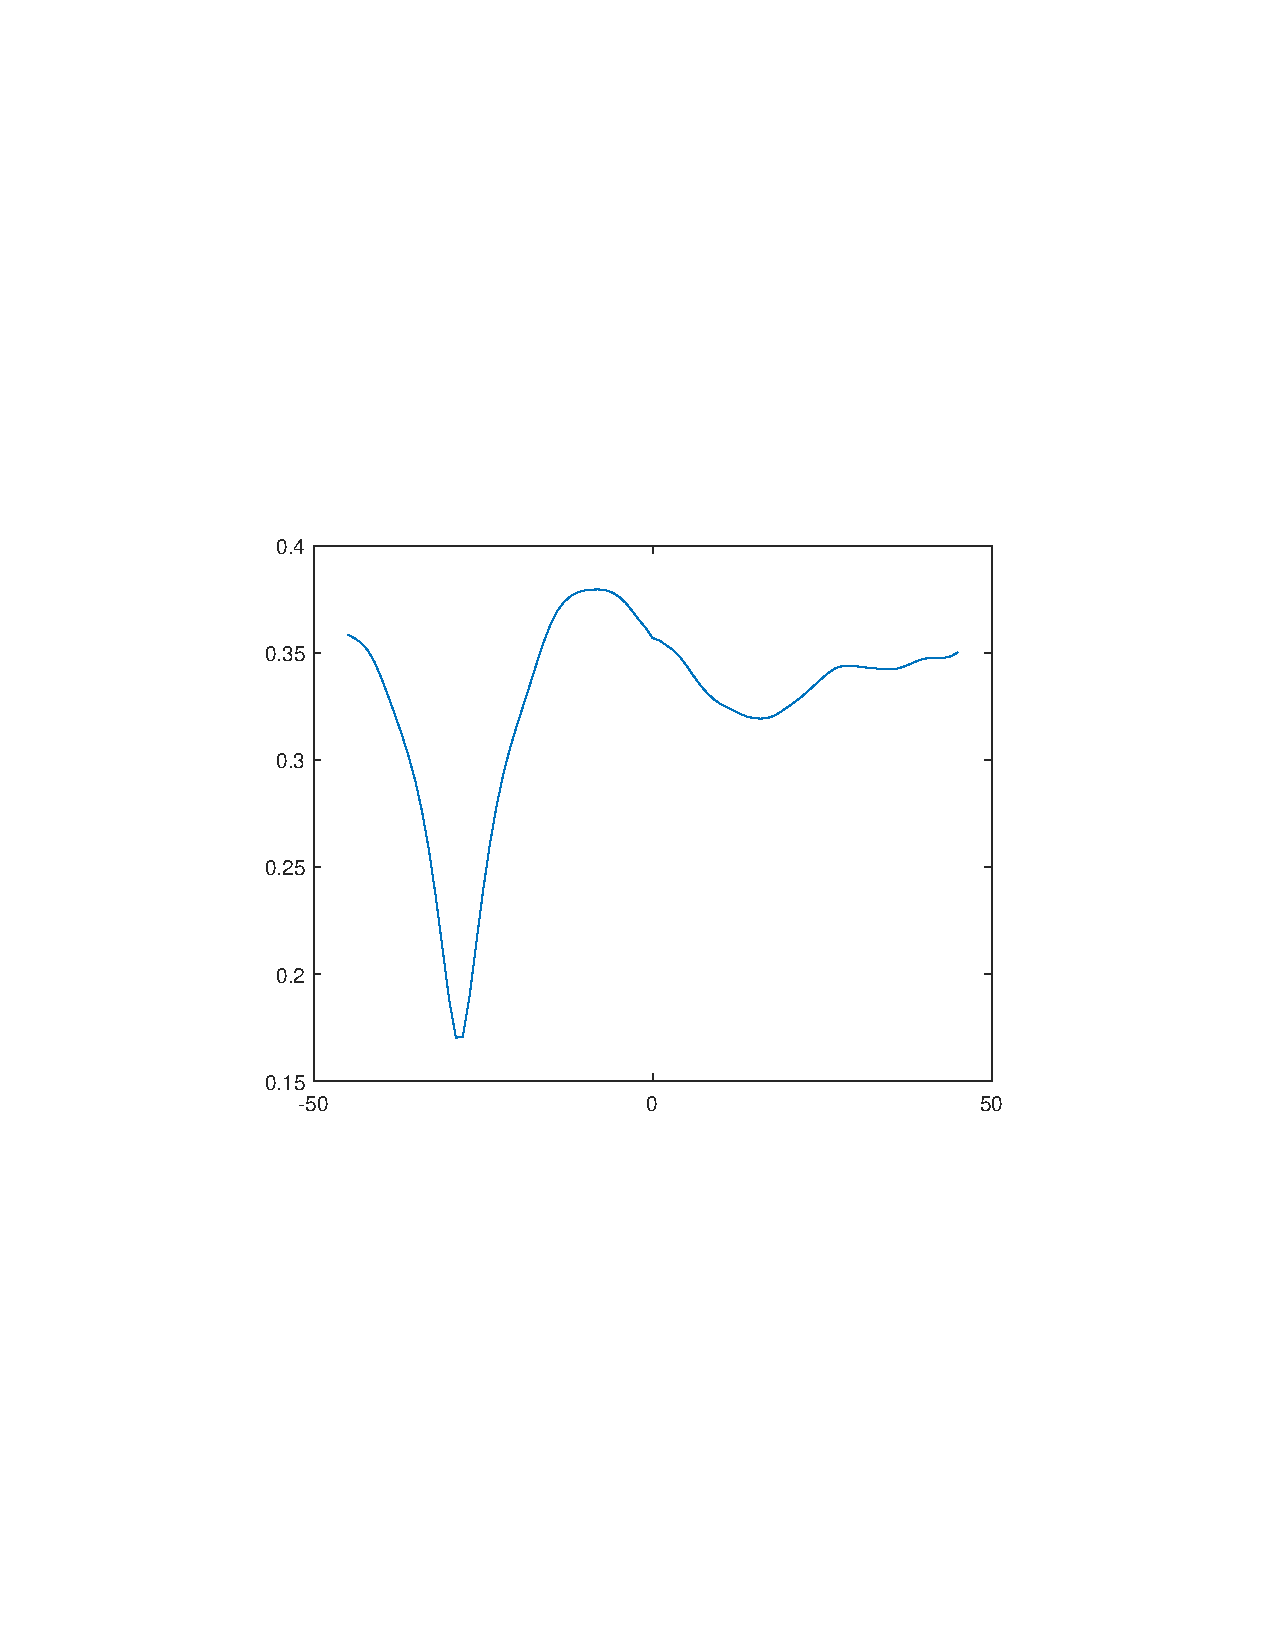
\includegraphics[scale=0.95]{ncc.pdf}
\caption{The graph of the NCC of $J1$ and $J4$ as a function of $\theta$.}
\end{figure}

\begin{figure}[H]
\centering
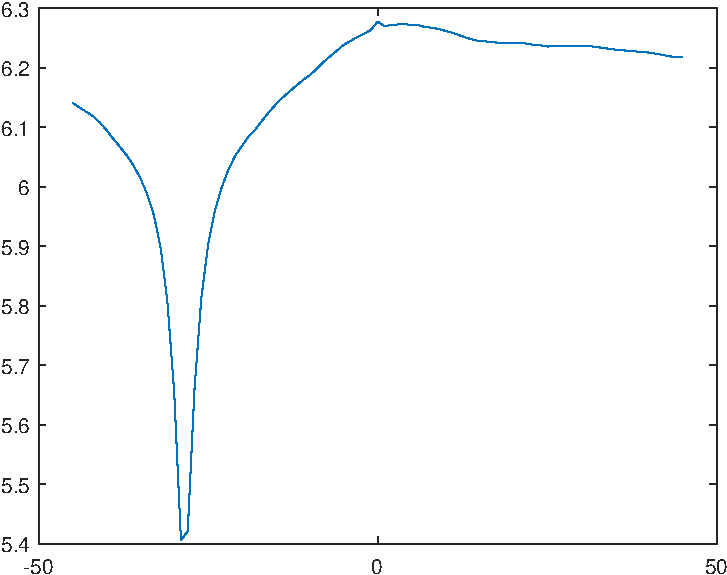
\includegraphics[scale=0.95]{je.pdf}
\caption{The graph of the JE of $J1$ and $J4$ as a function of $\theta$.}
\end{figure}

\begin{figure}[H]
\centering
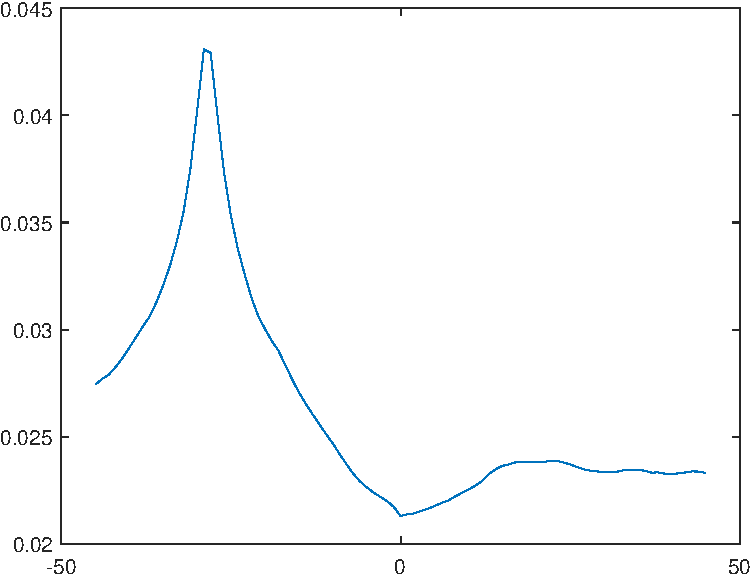
\includegraphics[scale=0.95]{qmi.pdf}
\caption{The graph of the QMI of $J1$ and $J4$ as a function of $\theta$.}
\end{figure}

\item Based on the NCC graph, the optimal rotation is $\theta = -8^\circ$. Based on the Joint Entropy graph and the QMI graph, the optimal rotation is $\theta = -29^\circ$.

\item Here is the joint histogram between $J1$ and $J4$:
\begin{figure}[H]
\centering
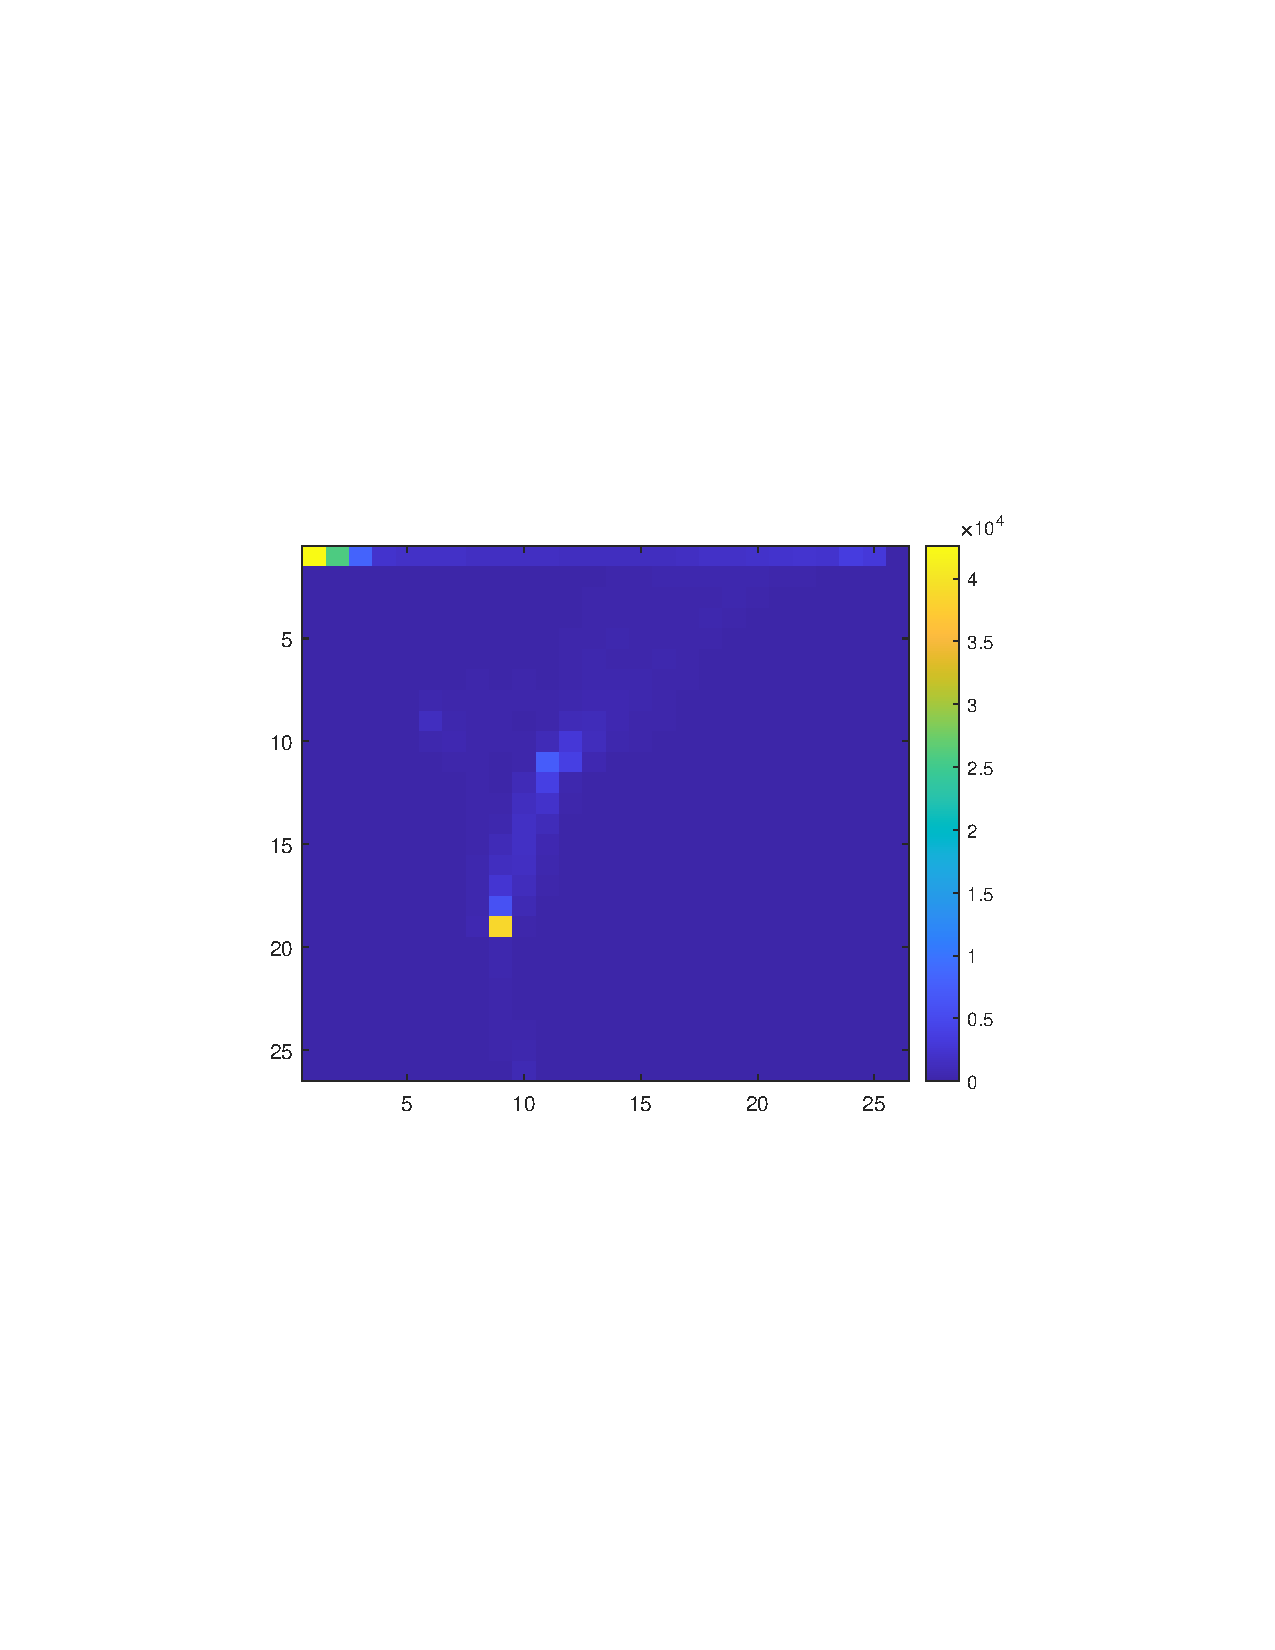
\includegraphics[scale=0.95]{histogram.pdf}
\caption{The joint histogram between images $J1$ and $J4$.}
\end{figure}

\item The intuition behind Quadratic Mutual Information (QMI)is simple: we want to quantify the amount of `mutual information' we have between the two images. That is, given the pixel intensity data in image $J1$, how much uncertainty (or dually, certainty) do we have about the corresponding pixel intensity data in image $J4$?

The reason for using quadratic terms is the same as the reason we use it for least squares: We don't want the errors to cancel out.

If we have high mutual information, that means that given some pixel intensity data in image $J1$, we can say with (relatively) high certainty what the corresponding pixel intensity data is in image $J4$.

The QMI is at its lowest when the random variables $I_1$ and $I_2$ are statistically independent. If we assume that $I_1$ and $I_2$ are statistically independent, then $p_{I_1 I_2}\big( i_1, i_2\big) = p_{I_1}\big( i_1\big)p_{I_2}\big( i_2\big)$, so we get
\begin{align*}
\text{QMI} &= \sum\limits_{i_1} \sum\limits_{i_2} \Big( p_{I_1 I_2}\big( i_1, i_2\big) - p_{I_1}\big( i_1\big)p_{I_2}\big( i_2\big) \Big)^2 \nonumber \\
&= \sum\limits_{i_1} \sum\limits_{i_2} \Big( p_{I_1}\big( i_1\big)p_{I_2}\big( i_2\big) - p_{I_1}\big( i_1\big)p_{I_2}\big( i_2\big) \Big)^2 \\
&= \sum\limits_{i_1} \sum\limits_{i_2} 0 \\
&= 0
\end{align*}

The intuitive reason for this is because $I_1$ and $I_2$ are independent, the pixel intensity data in the first image has no bearing on the pixel intensity data in the second image, so we have, loosely speaking, 0 `mutual information'.
\end{enumerate}
\end{document}